\documentclass{book}
\usepackage[a4paper,top=2.5cm,bottom=2.5cm,left=2.5cm,right=2.5cm]{geometry}
\usepackage{makeidx}
\usepackage{natbib}
\usepackage{graphicx}
\usepackage{multicol}
\usepackage{float}
\usepackage{listings}
\usepackage{color}
\usepackage{ifthen}
\usepackage[table]{xcolor}
\usepackage{textcomp}
\usepackage{alltt}
\usepackage{ifpdf}
\ifpdf
\usepackage[pdftex,
            pagebackref=true,
            colorlinks=true,
            linkcolor=blue,
            unicode
           ]{hyperref}
\else
\usepackage[ps2pdf,
            pagebackref=true,
            colorlinks=true,
            linkcolor=blue,
            unicode
           ]{hyperref}
\usepackage{pspicture}
\fi
\usepackage[utf8]{inputenc}
\usepackage{mathptmx}
\usepackage[scaled=.90]{helvet}
\usepackage{courier}
\usepackage{sectsty}
\usepackage{amssymb}
\usepackage[titles]{tocloft}
\usepackage{doxygen}
\lstset{language=C++,inputencoding=utf8,basicstyle=\footnotesize,breaklines=true,breakatwhitespace=true,tabsize=4,numbers=left }
\makeindex
\setcounter{tocdepth}{3}
\renewcommand{\footrulewidth}{0.4pt}
\renewcommand{\familydefault}{\sfdefault}
\hfuzz=15pt
\setlength{\emergencystretch}{15pt}
\hbadness=750
\tolerance=750
\begin{document}
\hypersetup{pageanchor=false,citecolor=blue}
\begin{titlepage}
\vspace*{7cm}
\begin{center}
{\Large C\-O\-S110\-Project \\[1ex]\large 0.\-001a }\\
\vspace*{1cm}
{\large Generated by Doxygen 1.8.3.1}\\
\vspace*{0.5cm}
{\small Thu Sep 19 2013 12:33:03}\\
\end{center}
\end{titlepage}
\clearemptydoublepage
\pagenumbering{roman}
\tableofcontents
\clearemptydoublepage
\pagenumbering{arabic}
\hypersetup{pageanchor=true,citecolor=blue}
\chapter{Hierarchical Index}
\section{Class Hierarchy}
This inheritance list is sorted roughly, but not completely, alphabetically\-:\begin{DoxyCompactList}
\item \contentsline{section}{Ammo\-Unit}{\pageref{classAmmoUnit}}{}
\begin{DoxyCompactList}
\item \contentsline{section}{Assassin}{\pageref{classAssassin}}{}
\item \contentsline{section}{Ranger}{\pageref{classRanger}}{}
\end{DoxyCompactList}
\item \contentsline{section}{Game}{\pageref{classGame}}{}
\item \contentsline{section}{Map}{\pageref{classMap}}{}
\item pair\begin{DoxyCompactList}
\item \contentsline{section}{Coord}{\pageref{structCoord}}{}
\end{DoxyCompactList}
\item \contentsline{section}{Piece}{\pageref{classPiece}}{}
\begin{DoxyCompactList}
\item \contentsline{section}{Immovable\-Piece}{\pageref{classImmovablePiece}}{}
\begin{DoxyCompactList}
\item \contentsline{section}{Boulder}{\pageref{classBoulder}}{}
\item \contentsline{section}{Wall}{\pageref{classWall}}{}
\item \contentsline{section}{Waypoint}{\pageref{classWaypoint}}{}
\end{DoxyCompactList}
\item \contentsline{section}{Movable\-Piece}{\pageref{classMovablePiece}}{}
\begin{DoxyCompactList}
\item \contentsline{section}{Creep}{\pageref{classCreep}}{}
\begin{DoxyCompactList}
\item \contentsline{section}{Critter}{\pageref{classCritter}}{}
\item \contentsline{section}{Hammer}{\pageref{classHammer}}{}
\item \contentsline{section}{Hunter}{\pageref{classHunter}}{}
\item \contentsline{section}{Runner}{\pageref{classRunner}}{}
\item \contentsline{section}{Sleeper}{\pageref{classSleeper}}{}
\end{DoxyCompactList}
\item \contentsline{section}{Sprite}{\pageref{classSprite}}{}
\begin{DoxyCompactList}
\item \contentsline{section}{Melee\-Sprite}{\pageref{classMeleeSprite}}{}
\begin{DoxyCompactList}
\item \contentsline{section}{Assassin}{\pageref{classAssassin}}{}
\item \contentsline{section}{Warrior}{\pageref{classWarrior}}{}
\end{DoxyCompactList}
\item \contentsline{section}{Ranged\-Sprite}{\pageref{classRangedSprite}}{}
\begin{DoxyCompactList}
\item \contentsline{section}{Mage}{\pageref{classMage}}{}
\item \contentsline{section}{Ranger}{\pageref{classRanger}}{}
\end{DoxyCompactList}
\end{DoxyCompactList}
\end{DoxyCompactList}
\end{DoxyCompactList}
\item \contentsline{section}{Player}{\pageref{classPlayer}}{}
\end{DoxyCompactList}

\chapter{Class Index}
\section{Class List}
Here are the classes, structs, unions and interfaces with brief descriptions\-:\begin{DoxyCompactList}
\item\contentsline{section}{\hyperlink{classAmmoUnit}{Ammo\-Unit} }{\pageref{classAmmoUnit}}{}
\item\contentsline{section}{\hyperlink{classAssassin}{Assassin} }{\pageref{classAssassin}}{}
\item\contentsline{section}{\hyperlink{classBoulder}{Boulder} }{\pageref{classBoulder}}{}
\item\contentsline{section}{\hyperlink{structCoord}{Coord} \\*Struct to hold coordinates of objects in the \hyperlink{classMap}{Map} }{\pageref{structCoord}}{}
\item\contentsline{section}{\hyperlink{classCreep}{Creep} }{\pageref{classCreep}}{}
\item\contentsline{section}{\hyperlink{classCritter}{Critter} }{\pageref{classCritter}}{}
\item\contentsline{section}{\hyperlink{classGame}{Game} }{\pageref{classGame}}{}
\item\contentsline{section}{\hyperlink{classHammer}{Hammer} }{\pageref{classHammer}}{}
\item\contentsline{section}{\hyperlink{classHunter}{Hunter} }{\pageref{classHunter}}{}
\item\contentsline{section}{\hyperlink{classImmovablePiece}{Immovable\-Piece} }{\pageref{classImmovablePiece}}{}
\item\contentsline{section}{\hyperlink{classMage}{Mage} }{\pageref{classMage}}{}
\item\contentsline{section}{\hyperlink{classMap}{Map} \\*The \hyperlink{classMap}{Map} class }{\pageref{classMap}}{}
\item\contentsline{section}{\hyperlink{classMeleeSprite}{Melee\-Sprite} }{\pageref{classMeleeSprite}}{}
\item\contentsline{section}{\hyperlink{classMovablePiece}{Movable\-Piece} }{\pageref{classMovablePiece}}{}
\item\contentsline{section}{\hyperlink{classPiece}{Piece} }{\pageref{classPiece}}{}
\item\contentsline{section}{\hyperlink{classPlayer}{Player} }{\pageref{classPlayer}}{}
\item\contentsline{section}{\hyperlink{classRangedSprite}{Ranged\-Sprite} }{\pageref{classRangedSprite}}{}
\item\contentsline{section}{\hyperlink{classRanger}{Ranger} }{\pageref{classRanger}}{}
\item\contentsline{section}{\hyperlink{classRunner}{Runner} }{\pageref{classRunner}}{}
\item\contentsline{section}{\hyperlink{classSleeper}{Sleeper} }{\pageref{classSleeper}}{}
\item\contentsline{section}{\hyperlink{classSprite}{Sprite} }{\pageref{classSprite}}{}
\item\contentsline{section}{\hyperlink{classWall}{Wall} }{\pageref{classWall}}{}
\item\contentsline{section}{\hyperlink{classWarrior}{Warrior} }{\pageref{classWarrior}}{}
\item\contentsline{section}{\hyperlink{classWaypoint}{Waypoint} }{\pageref{classWaypoint}}{}
\end{DoxyCompactList}

\chapter{Class Documentation}
\hypertarget{classAmmoUnit}{\section{Ammo\-Unit Class Reference}
\label{classAmmoUnit}\index{Ammo\-Unit@{Ammo\-Unit}}
}
Inheritance diagram for Ammo\-Unit\-:\begin{figure}[H]
\begin{center}
\leavevmode
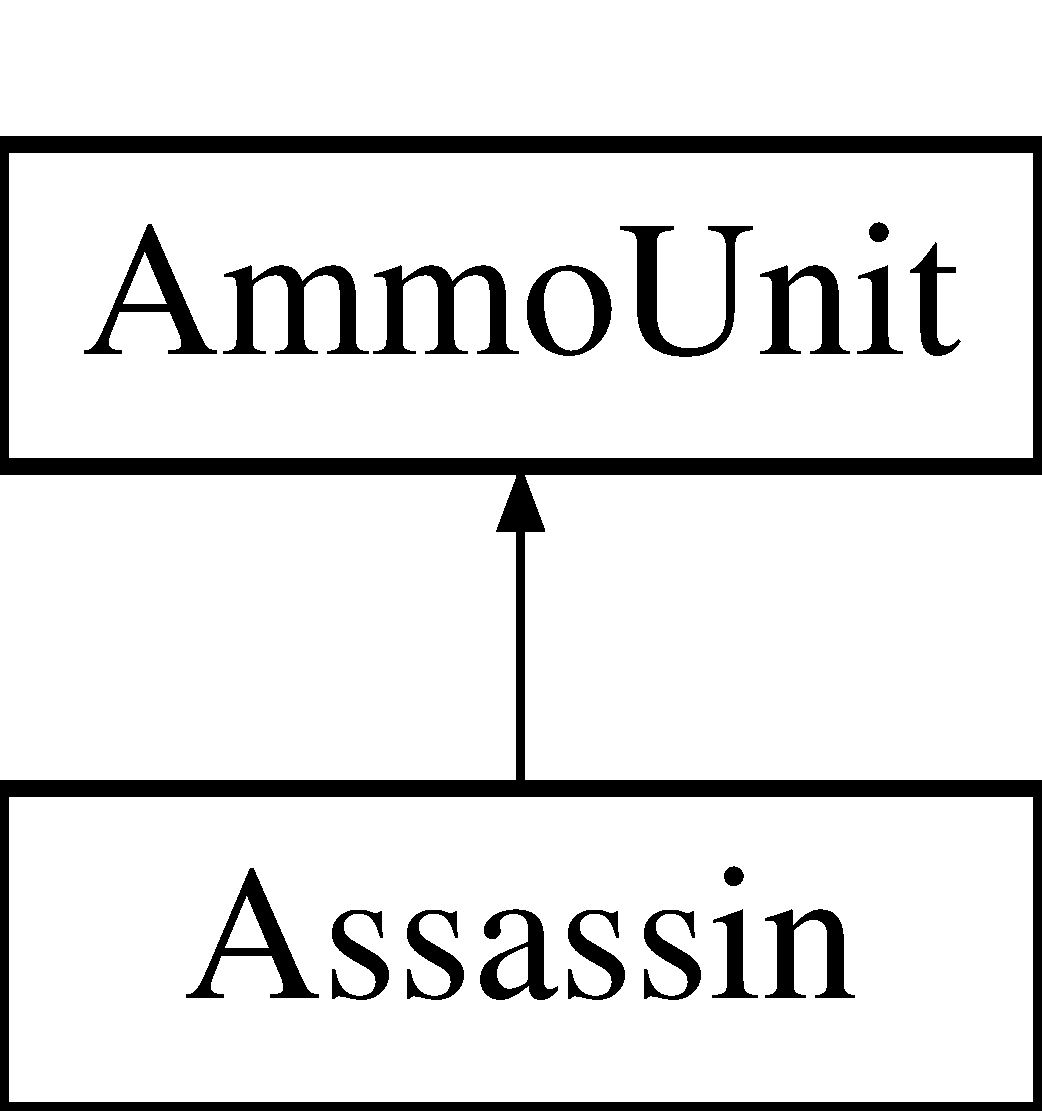
\includegraphics[height=2.000000cm]{classAmmoUnit}
\end{center}
\end{figure}


The documentation for this class was generated from the following file\-:\begin{DoxyCompactItemize}
\item 
/home/tom/\-Documents/\-Dev/\-C\-O\-S110\-\_\-\-Project/src/Ammo\-Unit.\-h\end{DoxyCompactItemize}

\hypertarget{classAssassin}{\section{Assassin Class Reference}
\label{classAssassin}\index{Assassin@{Assassin}}
}
Inheritance diagram for Assassin\-:\begin{figure}[H]
\begin{center}
\leavevmode
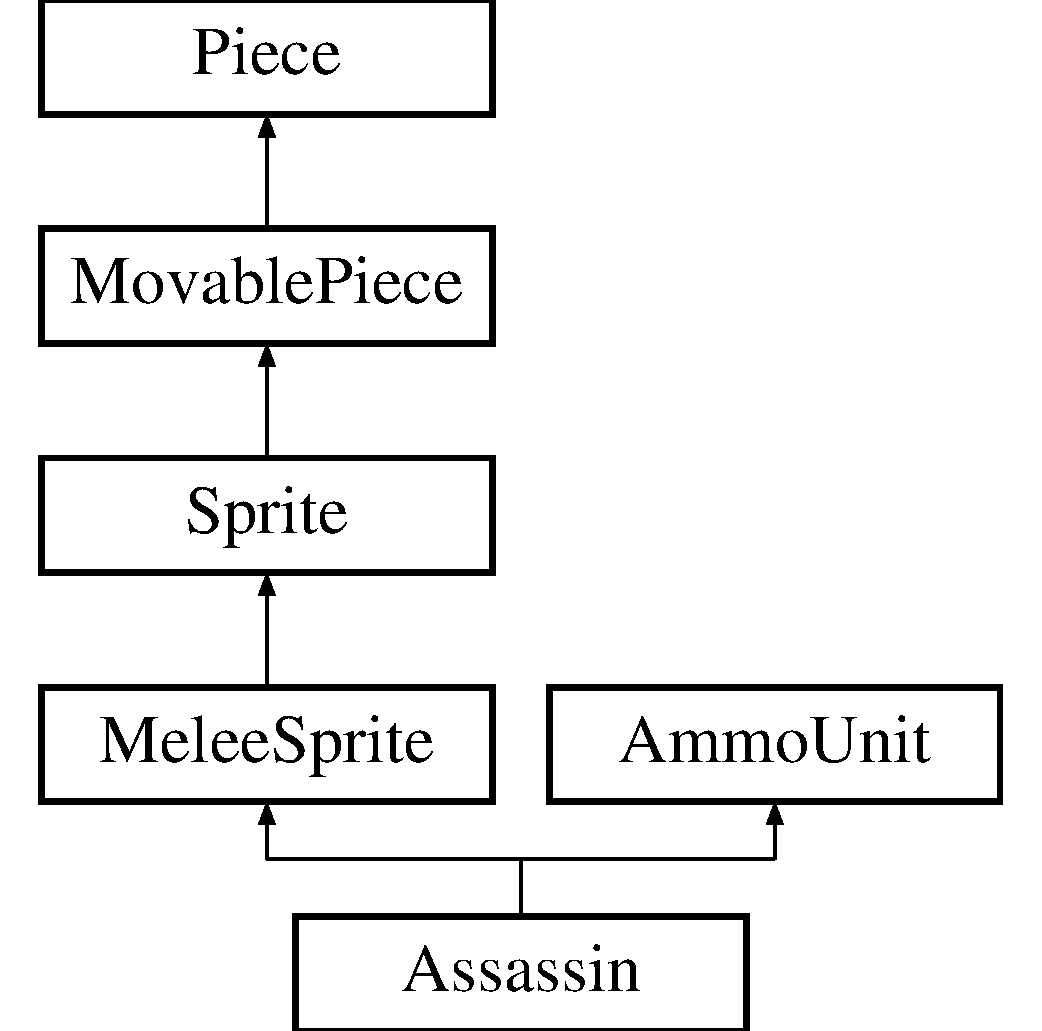
\includegraphics[height=5.000000cm]{classAssassin}
\end{center}
\end{figure}


The documentation for this class was generated from the following file\-:\begin{DoxyCompactItemize}
\item 
/home/tom/\-Documents/\-Dev/\-C\-O\-S110\-\_\-\-Project/src/Assassin.\-h\end{DoxyCompactItemize}

\hypertarget{classBoulder}{\section{Boulder Class Reference}
\label{classBoulder}\index{Boulder@{Boulder}}
}
Inheritance diagram for Boulder\-:\begin{figure}[H]
\begin{center}
\leavevmode
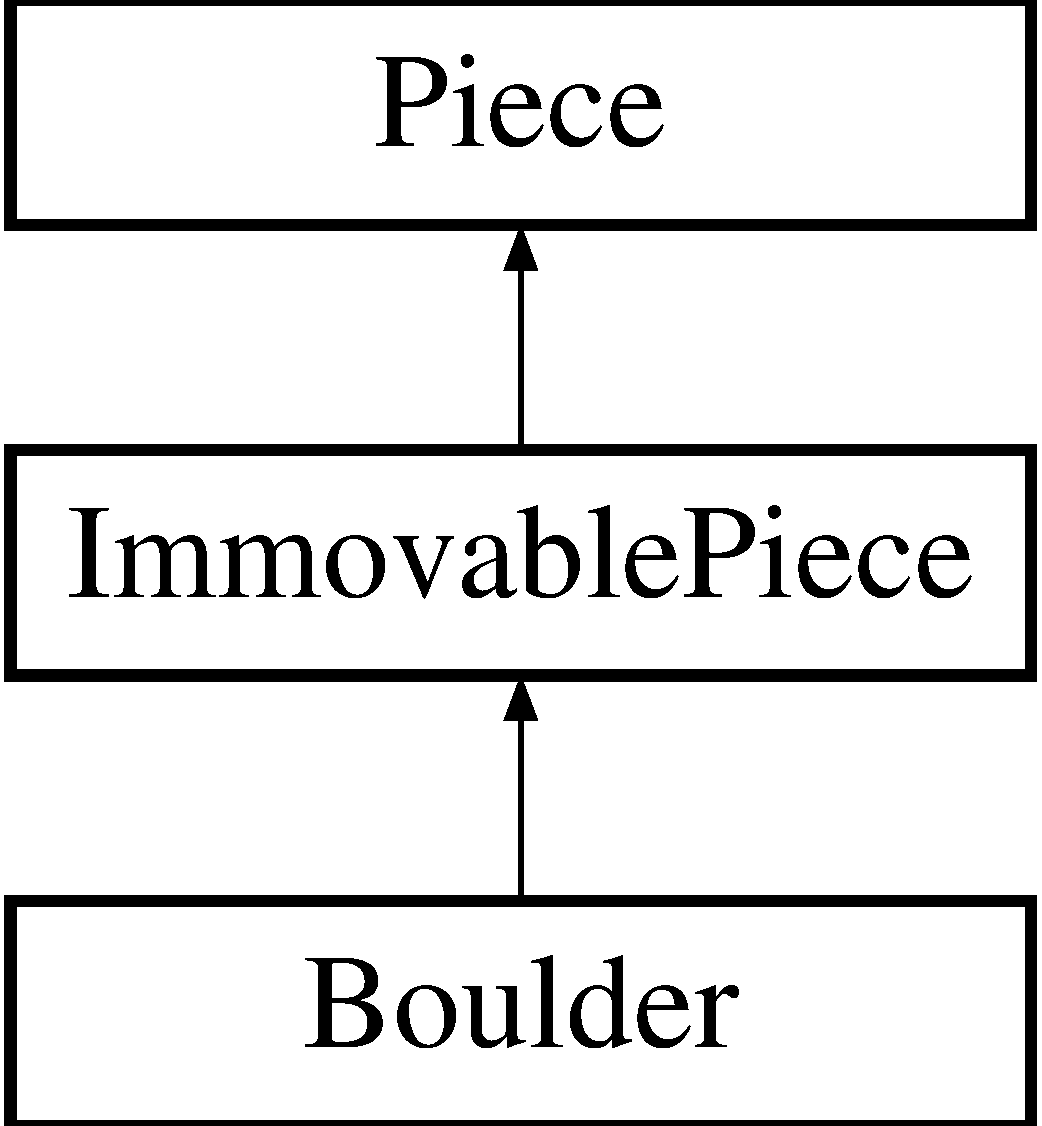
\includegraphics[height=3.000000cm]{classBoulder}
\end{center}
\end{figure}


The documentation for this class was generated from the following file\-:\begin{DoxyCompactItemize}
\item 
/home/tom/\-Documents/\-Dev/\-C\-O\-S110\-\_\-\-Project/src/Boulder.\-h\end{DoxyCompactItemize}

\hypertarget{structCoord}{\section{Coord Struct Reference}
\label{structCoord}\index{Coord@{Coord}}
}


Struct to hold coordinates of objects in the \hyperlink{classMap}{Map}.  




{\ttfamily \#include $<$Map.\-h$>$}

Inheritance diagram for Coord\-:\begin{figure}[H]
\begin{center}
\leavevmode
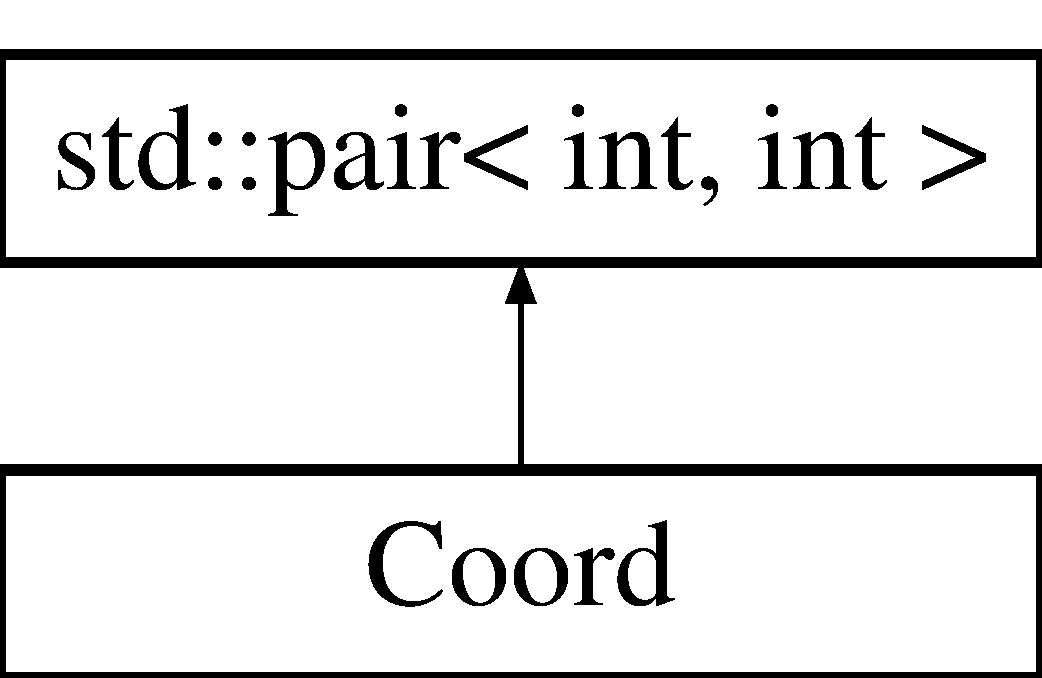
\includegraphics[height=2.000000cm]{structCoord}
\end{center}
\end{figure}
\subsection*{Public Member Functions}
\begin{DoxyCompactItemize}
\item 
int \& \hyperlink{structCoord_a685dd99f1e32d5e79f1fe6a7bbbceb76}{x} ()
\begin{DoxyCompactList}\small\item\em The x coordinate. \end{DoxyCompactList}\item 
int \& \hyperlink{structCoord_ab924c640df45524f31d54ee5c4870cbc}{y} ()
\begin{DoxyCompactList}\small\item\em The y coordinate. \end{DoxyCompactList}\end{DoxyCompactItemize}


\subsection{Detailed Description}
Struct to hold coordinates of objects in the \hyperlink{classMap}{Map}. 

This struct inherits from std\-::pair to enable the functionality that might be attractive in doing so.

Also, it keeps Lyle happy. He wanted the pair, and I wanted the struct. It's a middle-\/ground! \-:D Besides, Lyle, a pair is just a struct with some bolted-\/on stuffs anyway;

template $<$class T1, class T2$>$ struct pair; www.\-cplusplus.\-com/reference/utility/pair/ 



Use of this struct would be as follows;

\hyperlink{structCoord}{Coord} c;

c.\-x() = 4; c.\-y() = 5;

int x = c.\-x(); int y = c.\-y();

etc.

It's pretty nifty, yes? 

\subsection{Member Function Documentation}
\hypertarget{structCoord_a685dd99f1e32d5e79f1fe6a7bbbceb76}{\index{Coord@{Coord}!x@{x}}
\index{x@{x}!Coord@{Coord}}
\subsubsection[{x}]{\setlength{\rightskip}{0pt plus 5cm}int\& Coord\-::x (
\begin{DoxyParamCaption}
{}
\end{DoxyParamCaption}
)\hspace{0.3cm}{\ttfamily [inline]}}}\label{structCoord_a685dd99f1e32d5e79f1fe6a7bbbceb76}


The x coordinate. 

\begin{DoxyReturn}{Returns}
An integer reference. 
\end{DoxyReturn}
\hypertarget{structCoord_ab924c640df45524f31d54ee5c4870cbc}{\index{Coord@{Coord}!y@{y}}
\index{y@{y}!Coord@{Coord}}
\subsubsection[{y}]{\setlength{\rightskip}{0pt plus 5cm}int\& Coord\-::y (
\begin{DoxyParamCaption}
{}
\end{DoxyParamCaption}
)\hspace{0.3cm}{\ttfamily [inline]}}}\label{structCoord_ab924c640df45524f31d54ee5c4870cbc}


The y coordinate. 

\begin{DoxyReturn}{Returns}
An integer reference. 
\end{DoxyReturn}


The documentation for this struct was generated from the following file\-:\begin{DoxyCompactItemize}
\item 
/home/tom/\-Documents/\-Dev/\-C\-O\-S110\-\_\-\-Project/src/Map.\-h\end{DoxyCompactItemize}

\hypertarget{classCreep}{\section{Creep Class Reference}
\label{classCreep}\index{Creep@{Creep}}
}
Inheritance diagram for Creep\-:\begin{figure}[H]
\begin{center}
\leavevmode
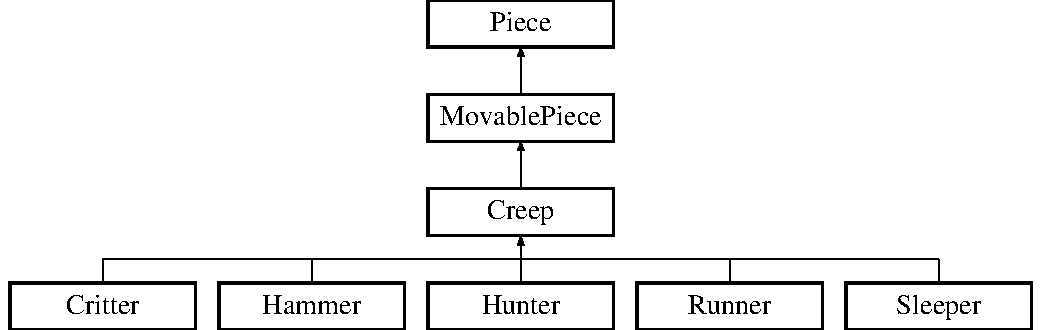
\includegraphics[height=4.000000cm]{classCreep}
\end{center}
\end{figure}


The documentation for this class was generated from the following file\-:\begin{DoxyCompactItemize}
\item 
/home/tom/\-Documents/\-Dev/\-C\-O\-S110\-\_\-\-Project/src/Creep.\-h\end{DoxyCompactItemize}

\hypertarget{classCritter}{\section{Critter Class Reference}
\label{classCritter}\index{Critter@{Critter}}
}
Inheritance diagram for Critter\-:\begin{figure}[H]
\begin{center}
\leavevmode
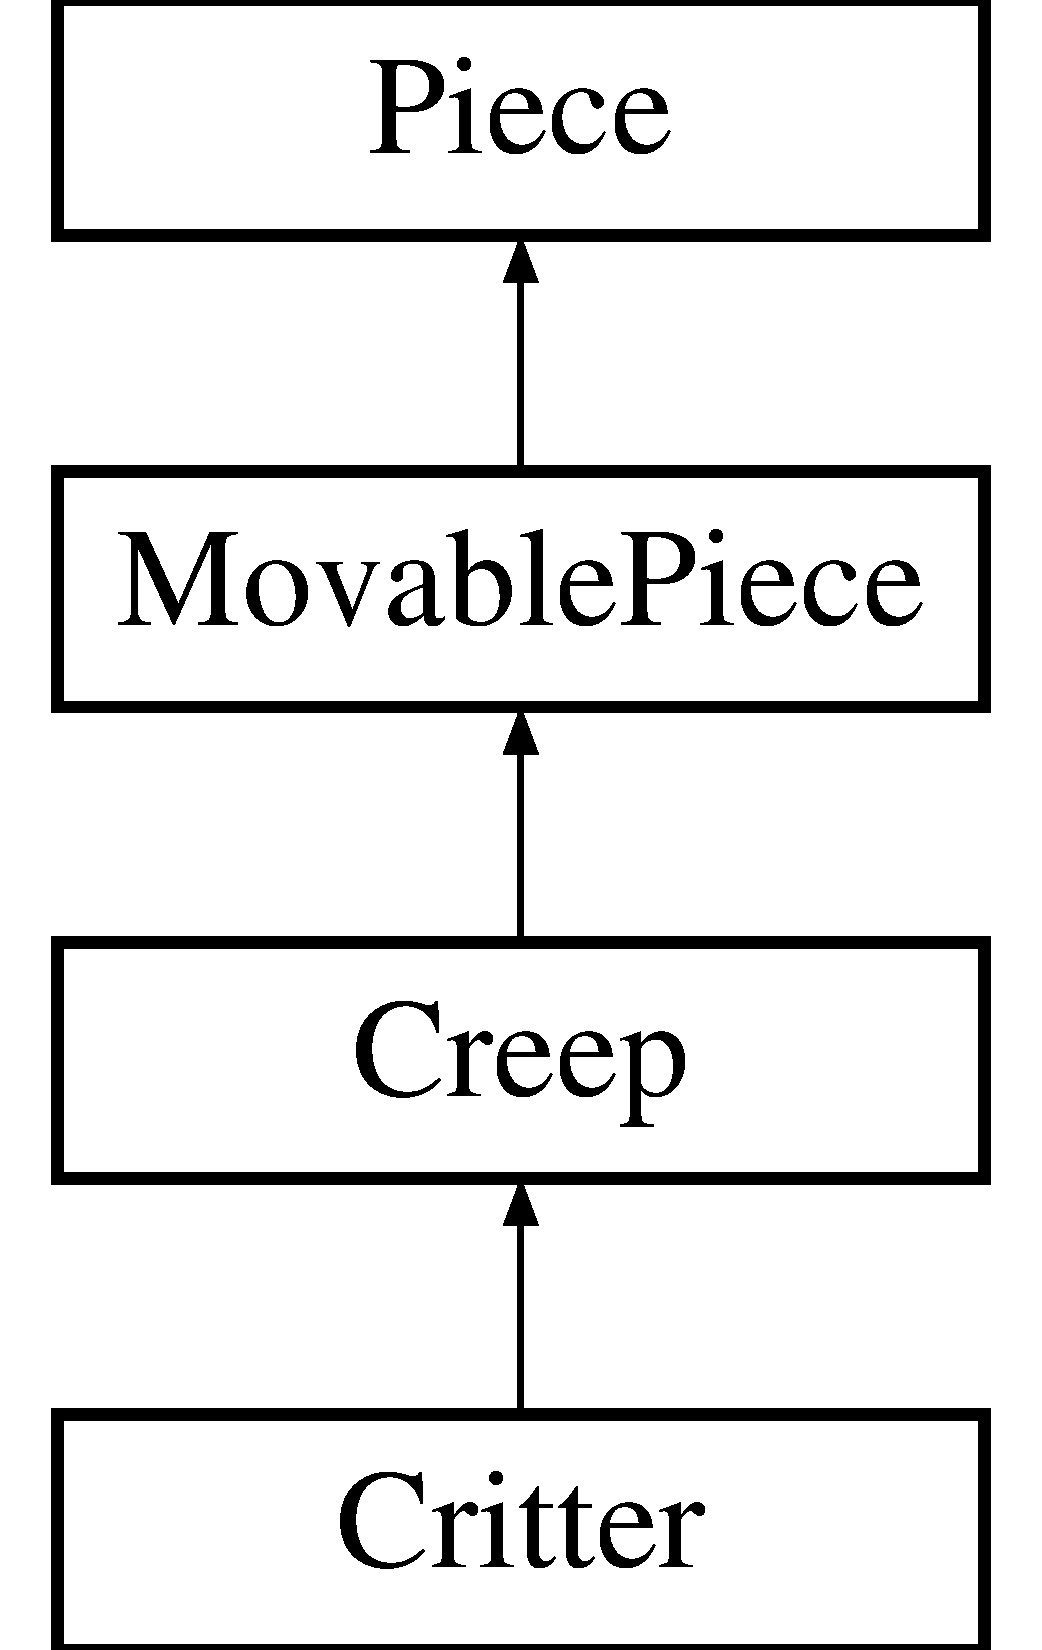
\includegraphics[height=4.000000cm]{classCritter}
\end{center}
\end{figure}


The documentation for this class was generated from the following file\-:\begin{DoxyCompactItemize}
\item 
/home/tom/\-Documents/\-Dev/\-C\-O\-S110\-\_\-\-Project/src/Critter.\-h\end{DoxyCompactItemize}

\hypertarget{classGame}{\section{Game Class Reference}
\label{classGame}\index{Game@{Game}}
}


The documentation for this class was generated from the following file\-:\begin{DoxyCompactItemize}
\item 
/home/tom/\-Documents/\-Dev/\-C\-O\-S110\-\_\-\-Project/src/Game.\-h\end{DoxyCompactItemize}

\hypertarget{classHammer}{\section{Hammer Class Reference}
\label{classHammer}\index{Hammer@{Hammer}}
}
Inheritance diagram for Hammer\-:\begin{figure}[H]
\begin{center}
\leavevmode
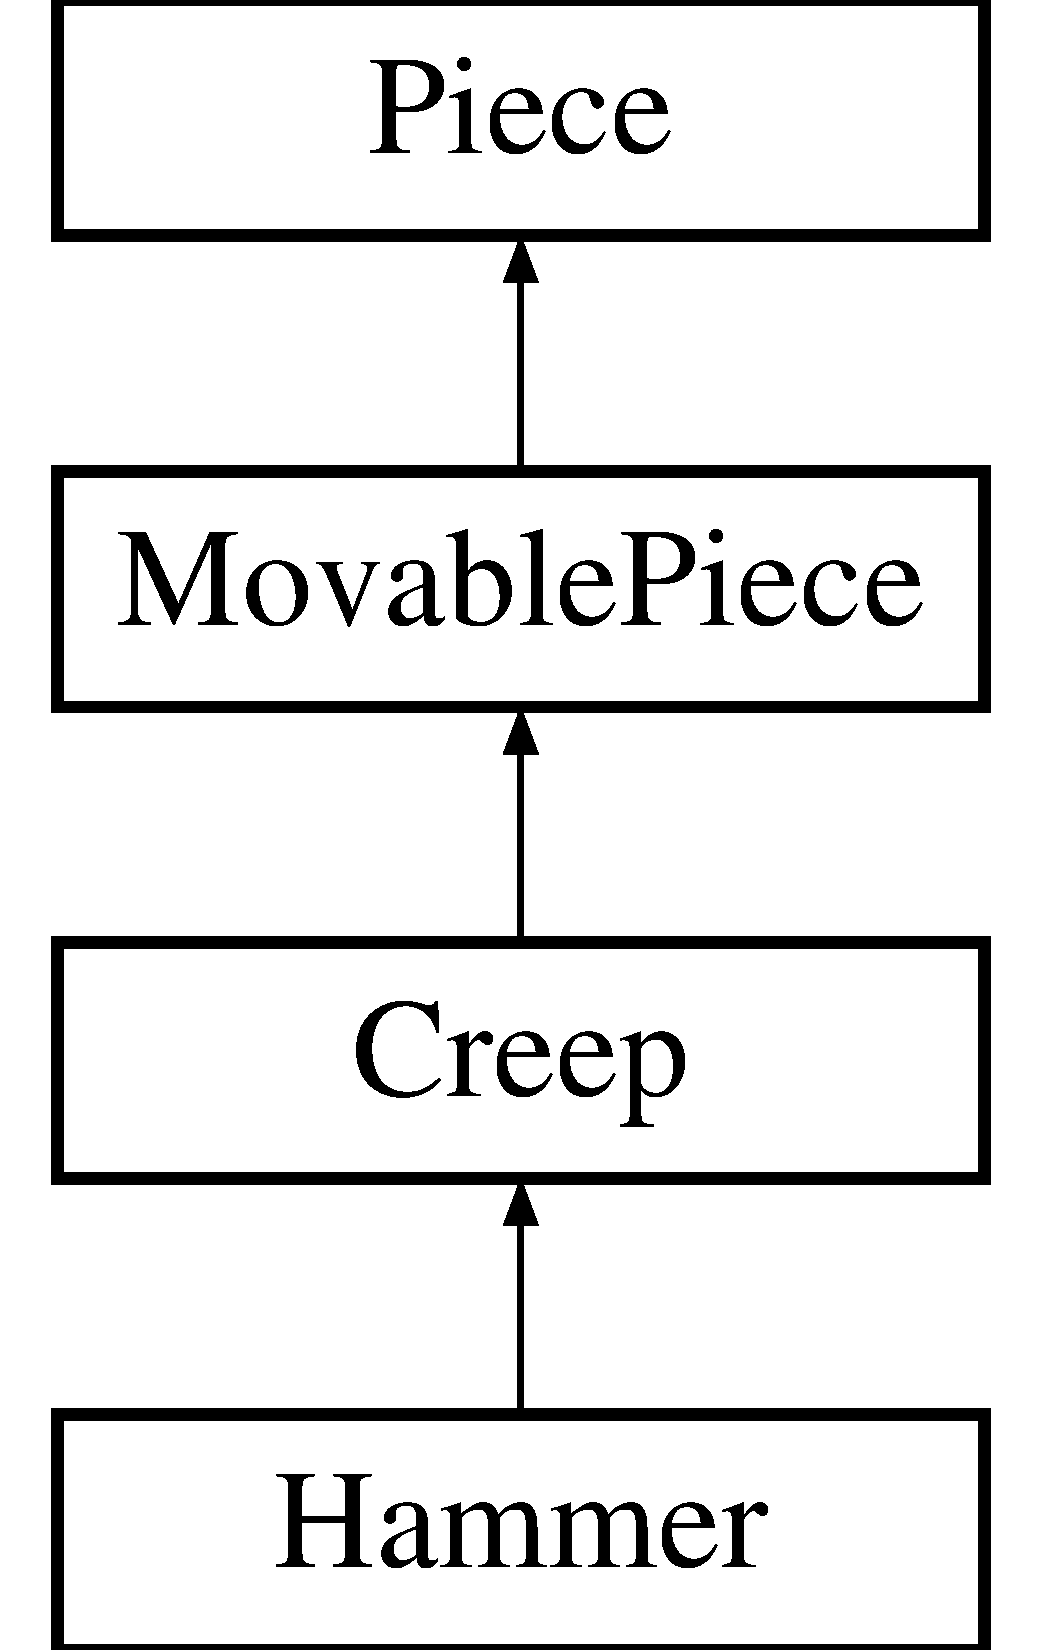
\includegraphics[height=4.000000cm]{classHammer}
\end{center}
\end{figure}


The documentation for this class was generated from the following file\-:\begin{DoxyCompactItemize}
\item 
/home/tom/\-Documents/\-Dev/\-C\-O\-S110\-\_\-\-Project/src/Hammer.\-h\end{DoxyCompactItemize}

\hypertarget{classHunter}{\section{Hunter Class Reference}
\label{classHunter}\index{Hunter@{Hunter}}
}
Inheritance diagram for Hunter\-:\begin{figure}[H]
\begin{center}
\leavevmode
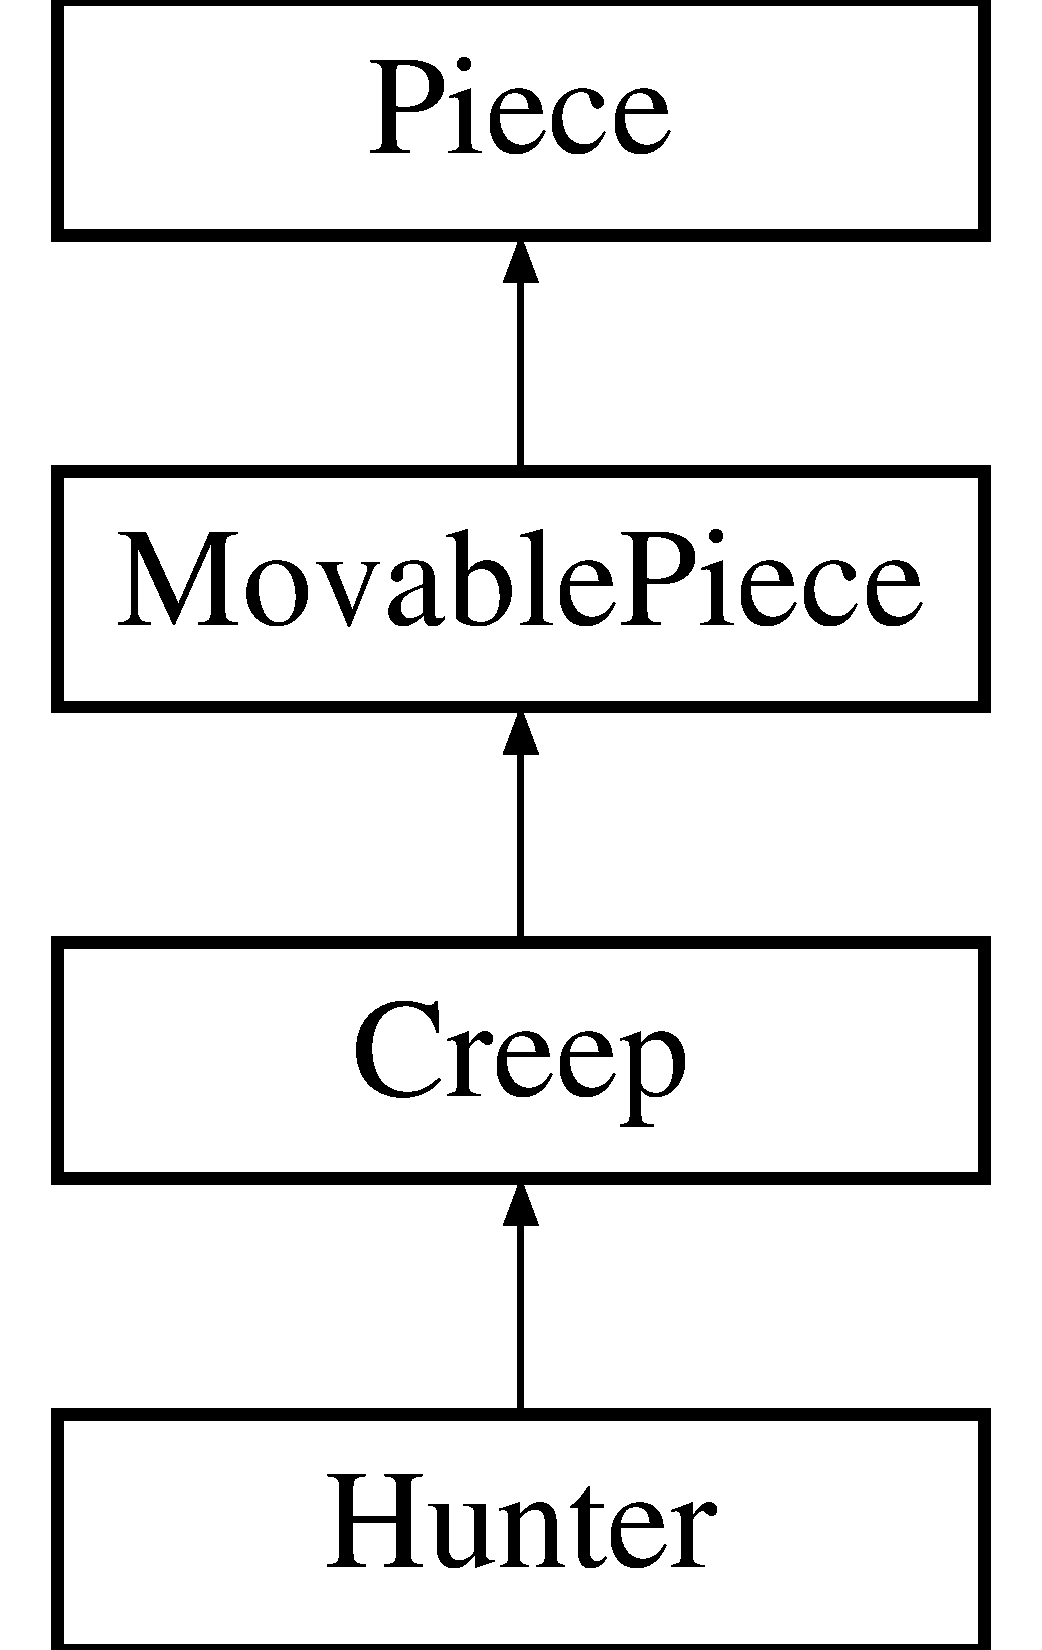
\includegraphics[height=4.000000cm]{classHunter}
\end{center}
\end{figure}


The documentation for this class was generated from the following file\-:\begin{DoxyCompactItemize}
\item 
/home/tom/\-Documents/\-Dev/\-C\-O\-S110\-\_\-\-Project/src/Hunter.\-h\end{DoxyCompactItemize}

\hypertarget{classImmovablePiece}{\section{Immovable\-Piece Class Reference}
\label{classImmovablePiece}\index{Immovable\-Piece@{Immovable\-Piece}}
}
Inheritance diagram for Immovable\-Piece\-:\begin{figure}[H]
\begin{center}
\leavevmode
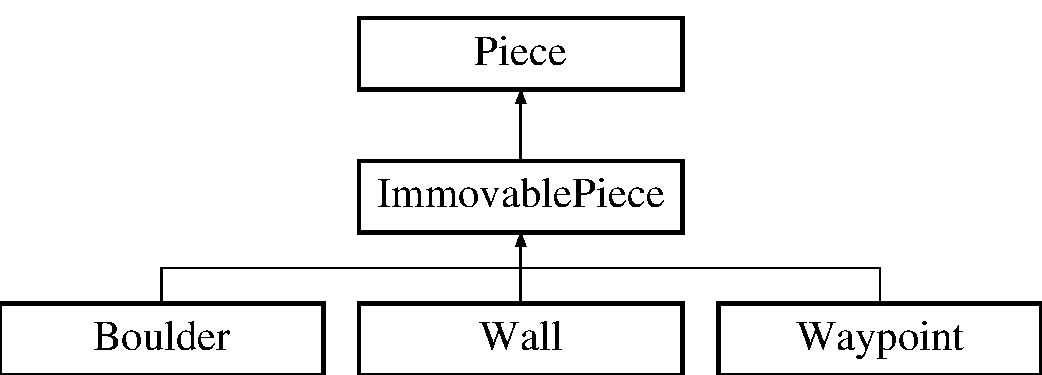
\includegraphics[height=3.000000cm]{classImmovablePiece}
\end{center}
\end{figure}


The documentation for this class was generated from the following file\-:\begin{DoxyCompactItemize}
\item 
/home/tom/\-Documents/\-Dev/\-C\-O\-S110\-\_\-\-Project/src/Immovable\-Piece.\-h\end{DoxyCompactItemize}

\hypertarget{classMage}{\section{Mage Class Reference}
\label{classMage}\index{Mage@{Mage}}
}
Inheritance diagram for Mage\-:\begin{figure}[H]
\begin{center}
\leavevmode
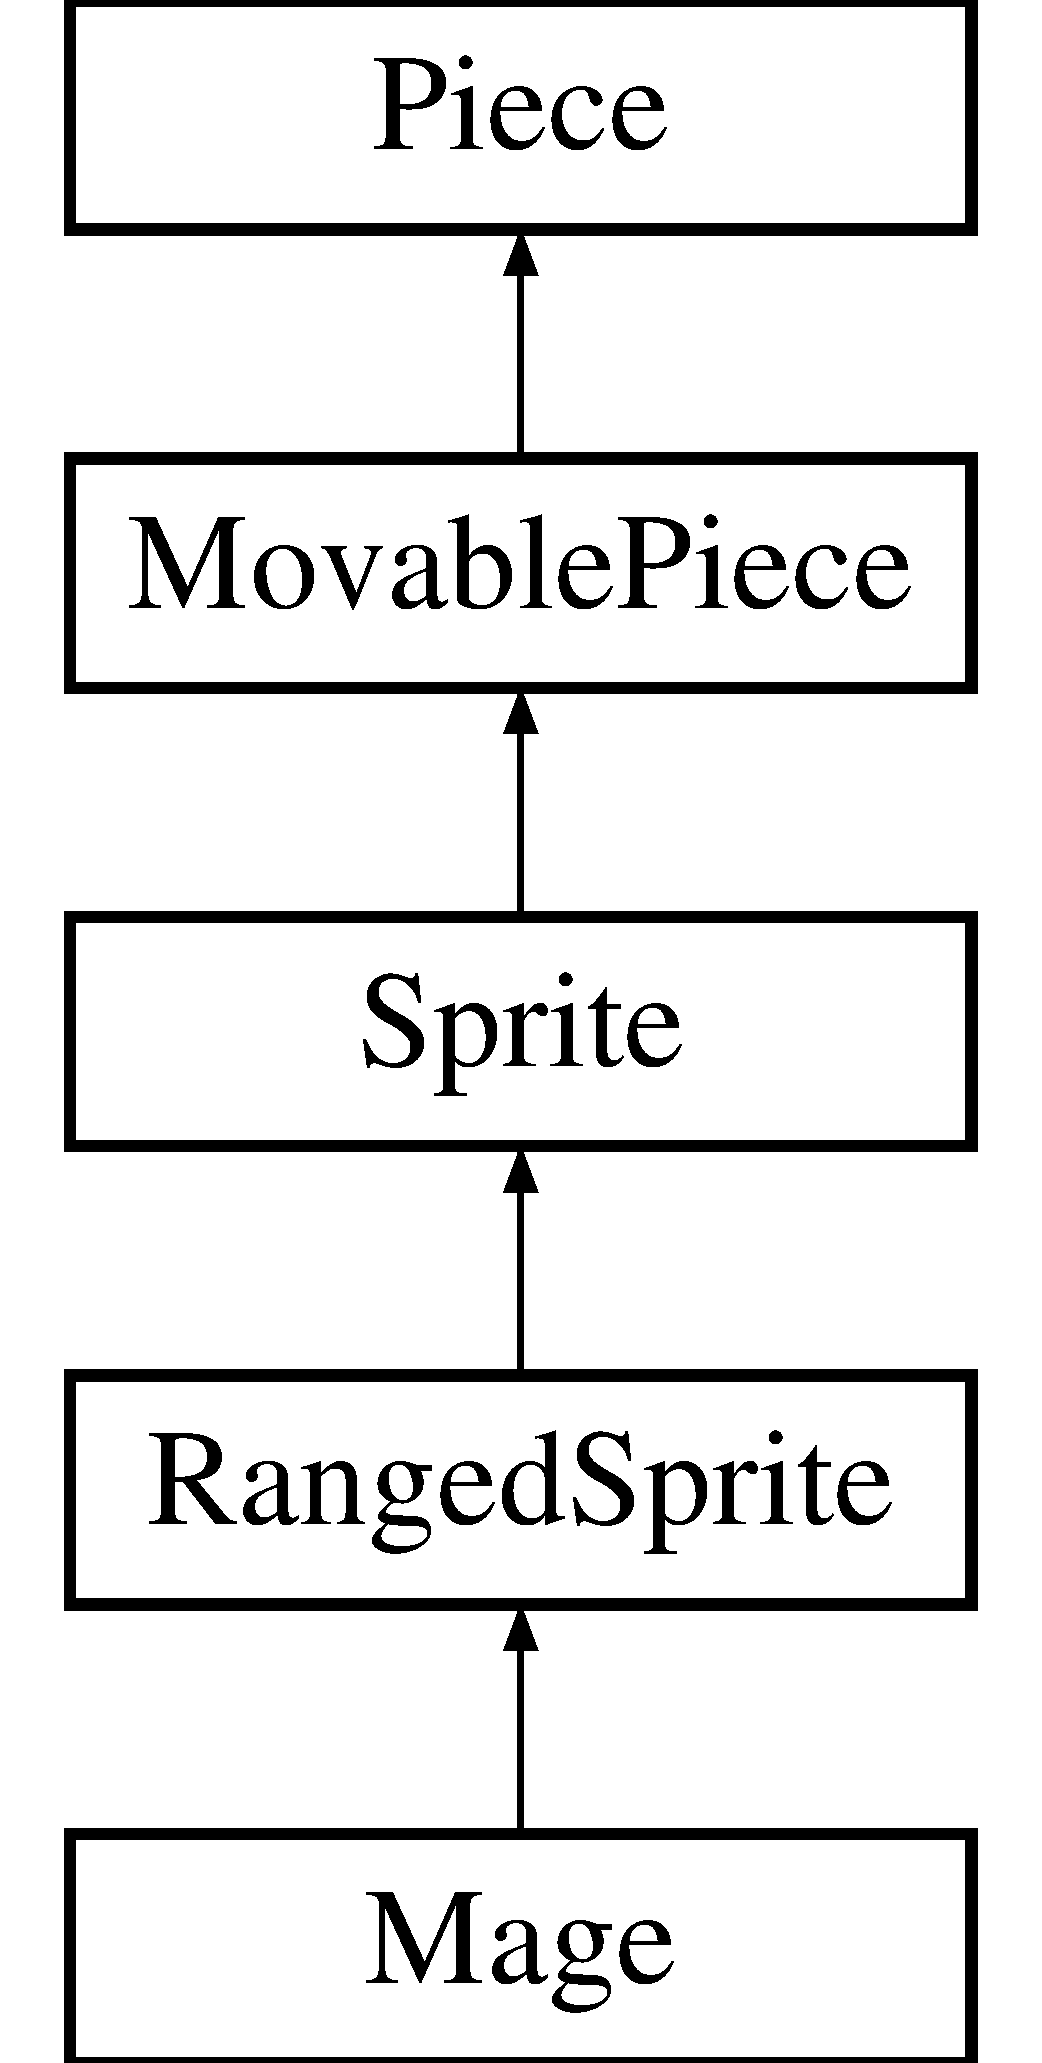
\includegraphics[height=5.000000cm]{classMage}
\end{center}
\end{figure}


The documentation for this class was generated from the following file\-:\begin{DoxyCompactItemize}
\item 
/home/tom/\-Documents/\-Dev/\-C\-O\-S110\-\_\-\-Project/src/Mage.\-h\end{DoxyCompactItemize}

\hypertarget{classMap}{\section{Map Class Reference}
\label{classMap}\index{Map@{Map}}
}


The \hyperlink{classMap}{Map} class.  




{\ttfamily \#include $<$Map.\-h$>$}

\subsection*{Public Member Functions}
\begin{DoxyCompactItemize}
\item 
bool \hyperlink{classMap_a2f7ddbd8a2830d766e4c6aa05451a537}{move} (const \hyperlink{structCoord}{Coord} \&from, const \hyperlink{structCoord}{Coord} \&to)
\begin{DoxyCompactList}\small\item\em Move the piece at the first coordinate on the map to the location of the second coordinate on the map. \end{DoxyCompactList}\item 
\hyperlink{structCoord}{Coord} $\ast$ \hyperlink{classMap_ae55dbf516d3caebb9572540e2bedcf5f}{get\-Sprite\-Relative\-Coord} (const \hyperlink{structCoord}{Coord} \&coord) const 
\begin{DoxyCompactList}\small\item\em Get the \hyperlink{classPlayer}{Player} \hyperlink{classSprite}{Sprite}'s relative coordinates to the provided coordinates. \end{DoxyCompactList}\item 
void \hyperlink{classMap_a0dffeac7daa5b0ea4c4f6f288926698c}{set\-Piece\-At} (const \hyperlink{classPiece}{Piece} $\ast$piece, const \hyperlink{structCoord}{Coord} \&coord)
\begin{DoxyCompactList}\small\item\em Set the piece at the coordinate on the map to the provided piece. \end{DoxyCompactList}\item 
\hyperlink{classPiece}{Piece} $\ast$ \hyperlink{classMap_aecc5a11d70fd7b77a829932632cbf107}{get\-Handle\-At} (const \hyperlink{structCoord}{Coord} \&coord) const 
\begin{DoxyCompactList}\small\item\em Get handle of piece at a coordinate on the map. \end{DoxyCompactList}\item 
void \hyperlink{classMap_ab12643cc3a8d5e48f566c1abb571e9bf}{update} ()
\begin{DoxyCompactList}\small\item\em Update the current state of the map. \end{DoxyCompactList}\end{DoxyCompactItemize}


\subsection{Detailed Description}
The \hyperlink{classMap}{Map} class. 

Holds the current state of the game's map as well as some functions to facilitate actions on the map itself. 

\subsection{Member Function Documentation}
\hypertarget{classMap_aecc5a11d70fd7b77a829932632cbf107}{\index{Map@{Map}!get\-Handle\-At@{get\-Handle\-At}}
\index{get\-Handle\-At@{get\-Handle\-At}!Map@{Map}}
\subsubsection[{get\-Handle\-At}]{\setlength{\rightskip}{0pt plus 5cm}{\bf Piece}$\ast$ Map\-::get\-Handle\-At (
\begin{DoxyParamCaption}
\item[{const {\bf Coord} \&}]{coord}
\end{DoxyParamCaption}
) const}}\label{classMap_aecc5a11d70fd7b77a829932632cbf107}


Get handle of piece at a coordinate on the map. 

Might need to be a pointer, we'll see.


\begin{DoxyParams}{Parameters}
{\em coord} & a constant \hyperlink{structCoord}{Coord} reference. \\
\hline
\end{DoxyParams}
\begin{DoxyReturn}{Returns}
The \hyperlink{classPiece}{Piece} object at the coordinate on the map. 
\end{DoxyReturn}
\hypertarget{classMap_ae55dbf516d3caebb9572540e2bedcf5f}{\index{Map@{Map}!get\-Sprite\-Relative\-Coord@{get\-Sprite\-Relative\-Coord}}
\index{get\-Sprite\-Relative\-Coord@{get\-Sprite\-Relative\-Coord}!Map@{Map}}
\subsubsection[{get\-Sprite\-Relative\-Coord}]{\setlength{\rightskip}{0pt plus 5cm}{\bf Coord}$\ast$ Map\-::get\-Sprite\-Relative\-Coord (
\begin{DoxyParamCaption}
\item[{const {\bf Coord} \&}]{coord}
\end{DoxyParamCaption}
) const}}\label{classMap_ae55dbf516d3caebb9572540e2bedcf5f}


Get the \hyperlink{classPlayer}{Player} \hyperlink{classSprite}{Sprite}'s relative coordinates to the provided coordinates. 

Not as generic as it could be.


\begin{DoxyParams}{Parameters}
{\em coord} & a constant \hyperlink{structCoord}{Coord} reference. \\
\hline
\end{DoxyParams}
\begin{DoxyReturn}{Returns}
The relative coordinate to the \hyperlink{classPlayer}{Player}'s \hyperlink{classSprite}{Sprite} on the map. 
\end{DoxyReturn}
\hypertarget{classMap_a2f7ddbd8a2830d766e4c6aa05451a537}{\index{Map@{Map}!move@{move}}
\index{move@{move}!Map@{Map}}
\subsubsection[{move}]{\setlength{\rightskip}{0pt plus 5cm}bool Map\-::move (
\begin{DoxyParamCaption}
\item[{const {\bf Coord} \&}]{from, }
\item[{const {\bf Coord} \&}]{to}
\end{DoxyParamCaption}
)}}\label{classMap_a2f7ddbd8a2830d766e4c6aa05451a537}


Move the piece at the first coordinate on the map to the location of the second coordinate on the map. 

The function will perform the actual move on the map should the move be valid and possible, and then return true. Should the move not be valid and possible, the function will return false and not perform any moves.


\begin{DoxyParams}{Parameters}
{\em from} & a constant \hyperlink{structCoord}{Coord} reference. \\
\hline
{\em to} & a constant \hyperlink{structCoord}{Coord} reference. \\
\hline
\end{DoxyParams}
\begin{DoxyReturn}{Returns}
A boolean signifying whether or not the move is possible. 
\end{DoxyReturn}
\hypertarget{classMap_a0dffeac7daa5b0ea4c4f6f288926698c}{\index{Map@{Map}!set\-Piece\-At@{set\-Piece\-At}}
\index{set\-Piece\-At@{set\-Piece\-At}!Map@{Map}}
\subsubsection[{set\-Piece\-At}]{\setlength{\rightskip}{0pt plus 5cm}void Map\-::set\-Piece\-At (
\begin{DoxyParamCaption}
\item[{const {\bf Piece} $\ast$}]{piece, }
\item[{const {\bf Coord} \&}]{coord}
\end{DoxyParamCaption}
)}}\label{classMap_a0dffeac7daa5b0ea4c4f6f288926698c}


Set the piece at the coordinate on the map to the provided piece. 


\begin{DoxyParams}{Parameters}
{\em piece} & a constant \hyperlink{classPiece}{Piece} pointer. \\
\hline
{\em coord} & a constant \hyperlink{structCoord}{Coord} reference. \\
\hline
\end{DoxyParams}
\begin{DoxyReturn}{Returns}
void 
\end{DoxyReturn}
\hypertarget{classMap_ab12643cc3a8d5e48f566c1abb571e9bf}{\index{Map@{Map}!update@{update}}
\index{update@{update}!Map@{Map}}
\subsubsection[{update}]{\setlength{\rightskip}{0pt plus 5cm}void Map\-::update (
\begin{DoxyParamCaption}
{}
\end{DoxyParamCaption}
)}}\label{classMap_ab12643cc3a8d5e48f566c1abb571e9bf}


Update the current state of the map. 

This update performs any moves or actions necessary and updates the map accordingly before ending the function.

\begin{DoxyReturn}{Returns}
void 
\end{DoxyReturn}


The documentation for this class was generated from the following file\-:\begin{DoxyCompactItemize}
\item 
/home/tom/\-Documents/\-Dev/\-C\-O\-S110\-\_\-\-Project/src/Map.\-h\end{DoxyCompactItemize}

\hypertarget{classMeleeSprite}{\section{Melee\-Sprite Class Reference}
\label{classMeleeSprite}\index{Melee\-Sprite@{Melee\-Sprite}}
}
Inheritance diagram for Melee\-Sprite\-:\begin{figure}[H]
\begin{center}
\leavevmode
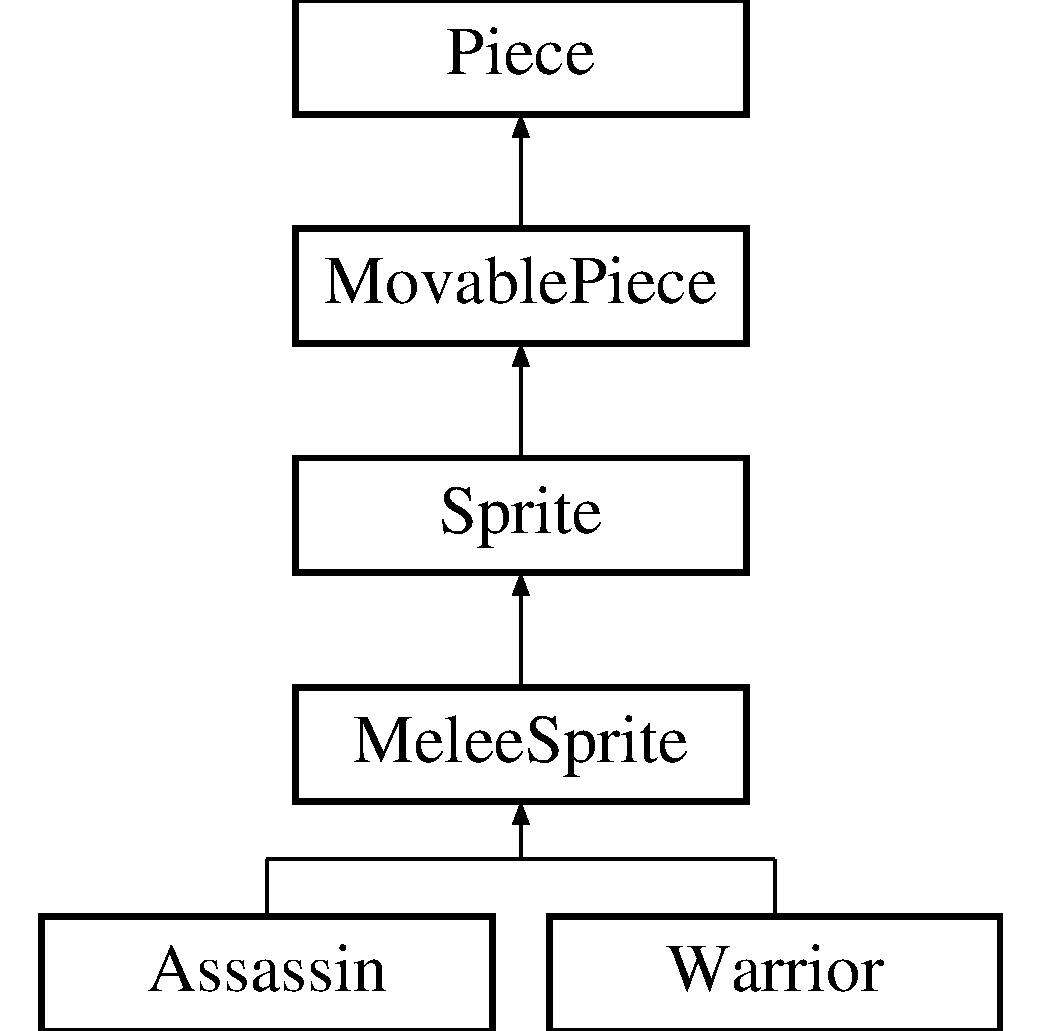
\includegraphics[height=5.000000cm]{classMeleeSprite}
\end{center}
\end{figure}


The documentation for this class was generated from the following file\-:\begin{DoxyCompactItemize}
\item 
/home/tom/\-Documents/\-Dev/\-C\-O\-S110\-\_\-\-Project/src/Melee\-Sprite.\-h\end{DoxyCompactItemize}

\hypertarget{classMovablePiece}{\section{Movable\-Piece Class Reference}
\label{classMovablePiece}\index{Movable\-Piece@{Movable\-Piece}}
}
Inheritance diagram for Movable\-Piece\-:\begin{figure}[H]
\begin{center}
\leavevmode
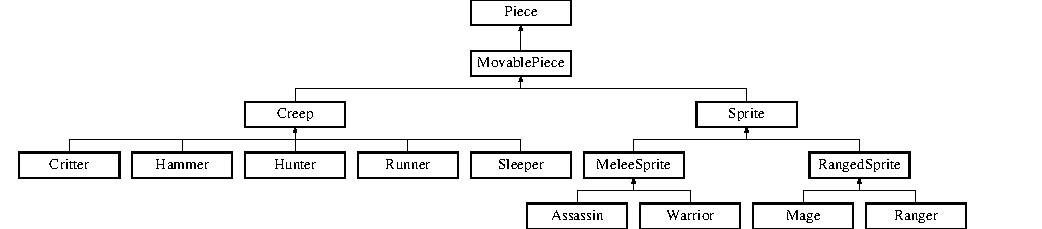
\includegraphics[height=3.080308cm]{classMovablePiece}
\end{center}
\end{figure}


The documentation for this class was generated from the following file\-:\begin{DoxyCompactItemize}
\item 
/home/tom/\-Documents/\-Dev/\-C\-O\-S110\-\_\-\-Project/src/Movable\-Piece.\-h\end{DoxyCompactItemize}

\hypertarget{classPiece}{\section{Piece Class Reference}
\label{classPiece}\index{Piece@{Piece}}
}
Inheritance diagram for Piece\-:\begin{figure}[H]
\begin{center}
\leavevmode
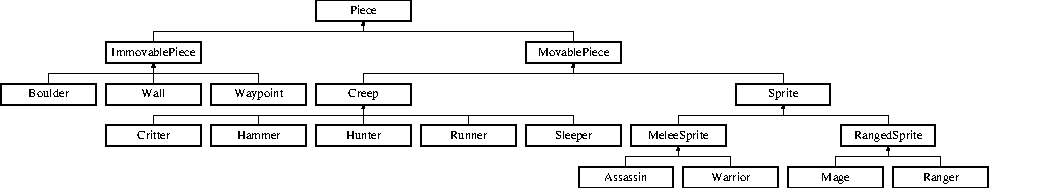
\includegraphics[height=2.522522cm]{classPiece}
\end{center}
\end{figure}


The documentation for this class was generated from the following file\-:\begin{DoxyCompactItemize}
\item 
/home/tom/\-Documents/\-Dev/\-C\-O\-S110\-\_\-\-Project/src/Piece.\-h\end{DoxyCompactItemize}

\hypertarget{classPlayer}{\section{Player Class Reference}
\label{classPlayer}\index{Player@{Player}}
}


The documentation for this class was generated from the following file\-:\begin{DoxyCompactItemize}
\item 
/home/tom/\-Documents/\-Dev/\-C\-O\-S110\-\_\-\-Project/src/Player.\-h\end{DoxyCompactItemize}

\hypertarget{classRangedSprite}{\section{Ranged\-Sprite Class Reference}
\label{classRangedSprite}\index{Ranged\-Sprite@{Ranged\-Sprite}}
}
Inheritance diagram for Ranged\-Sprite\-:\begin{figure}[H]
\begin{center}
\leavevmode
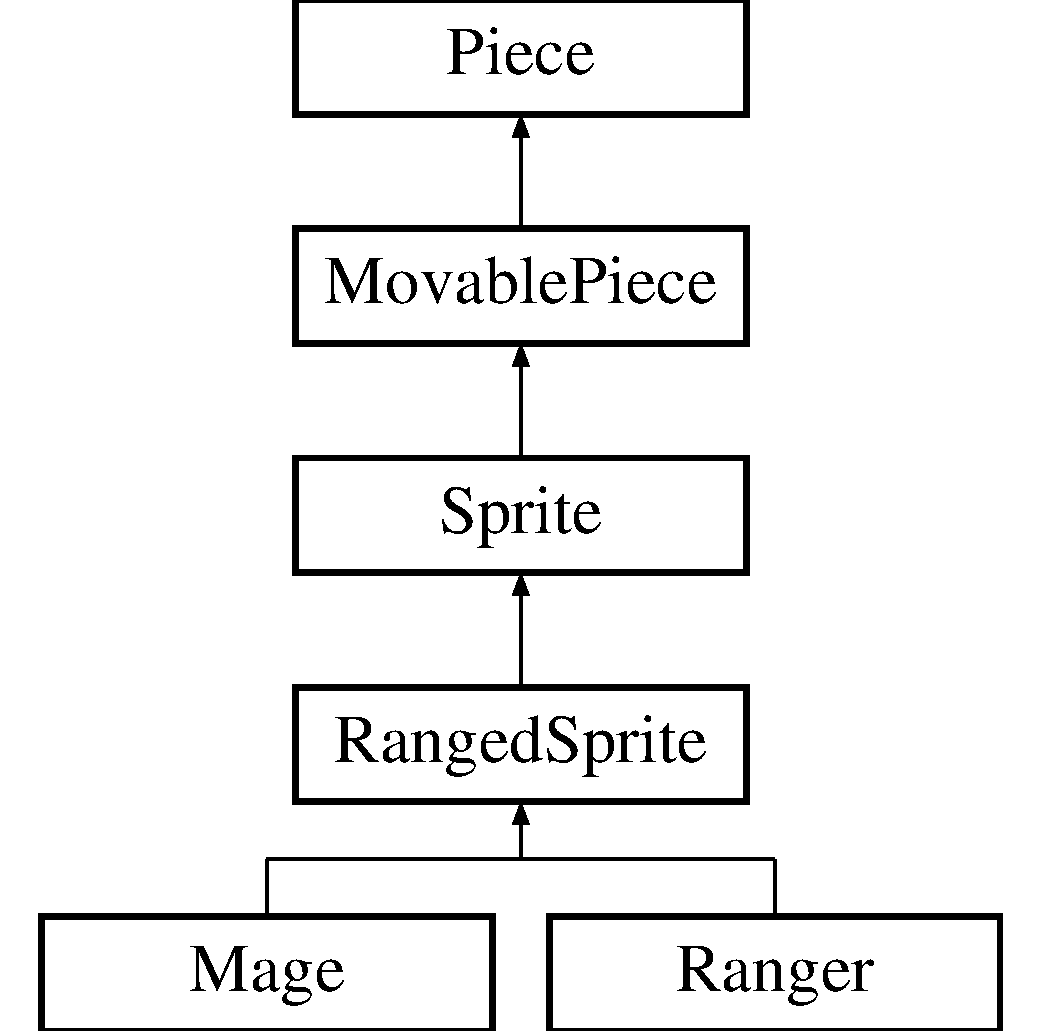
\includegraphics[height=5.000000cm]{classRangedSprite}
\end{center}
\end{figure}


The documentation for this class was generated from the following file\-:\begin{DoxyCompactItemize}
\item 
/home/tom/\-Documents/\-Dev/\-C\-O\-S110\-\_\-\-Project/src/Ranged\-Sprite.\-h\end{DoxyCompactItemize}

\hypertarget{classRanger}{\section{Ranger Class Reference}
\label{classRanger}\index{Ranger@{Ranger}}
}
Inheritance diagram for Ranger\-:\begin{figure}[H]
\begin{center}
\leavevmode
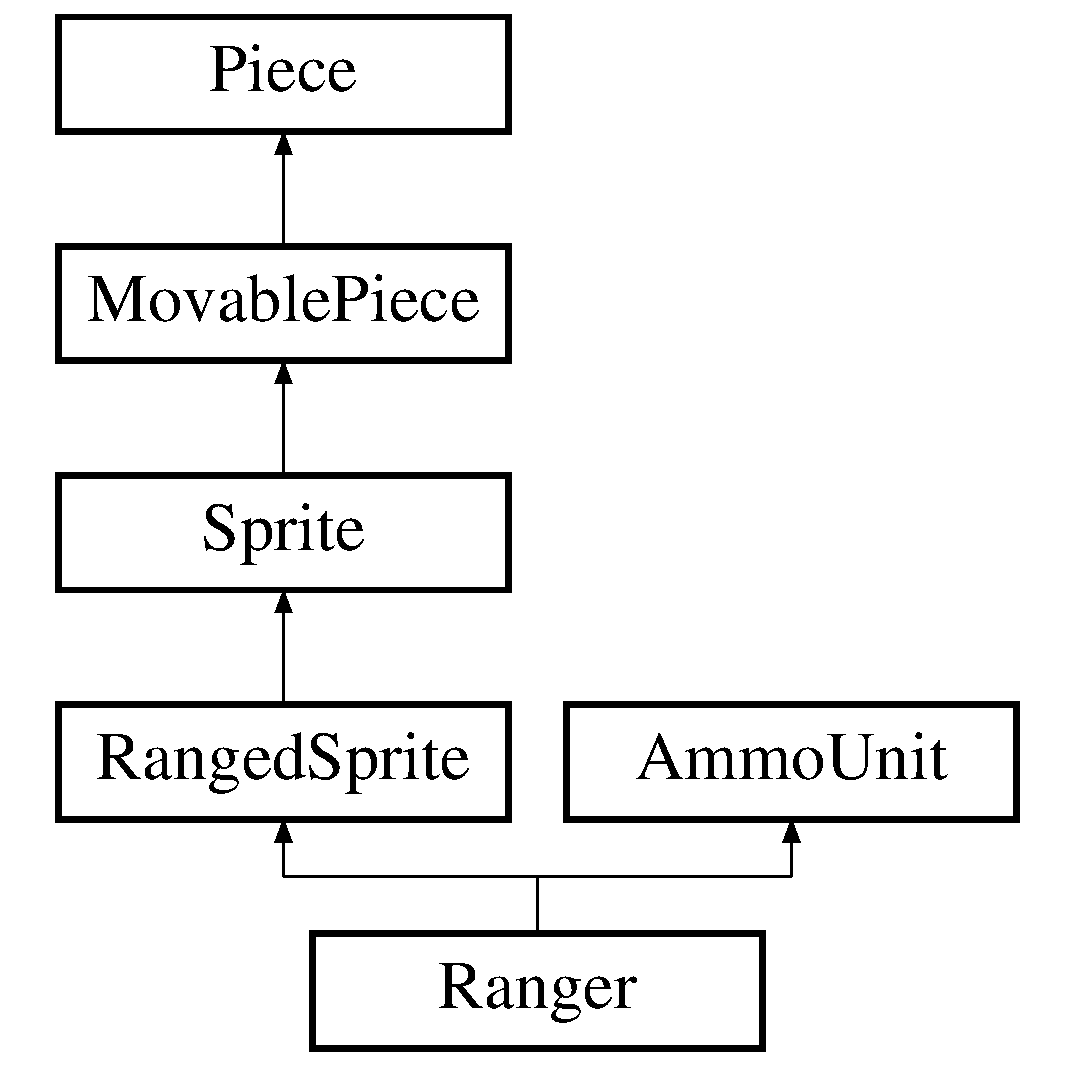
\includegraphics[height=5.000000cm]{classRanger}
\end{center}
\end{figure}


The documentation for this class was generated from the following file\-:\begin{DoxyCompactItemize}
\item 
/home/tom/\-Documents/\-Dev/\-C\-O\-S110\-\_\-\-Project/src/Ranger.\-h\end{DoxyCompactItemize}

\hypertarget{classRunner}{\section{Runner Class Reference}
\label{classRunner}\index{Runner@{Runner}}
}
Inheritance diagram for Runner\-:\begin{figure}[H]
\begin{center}
\leavevmode
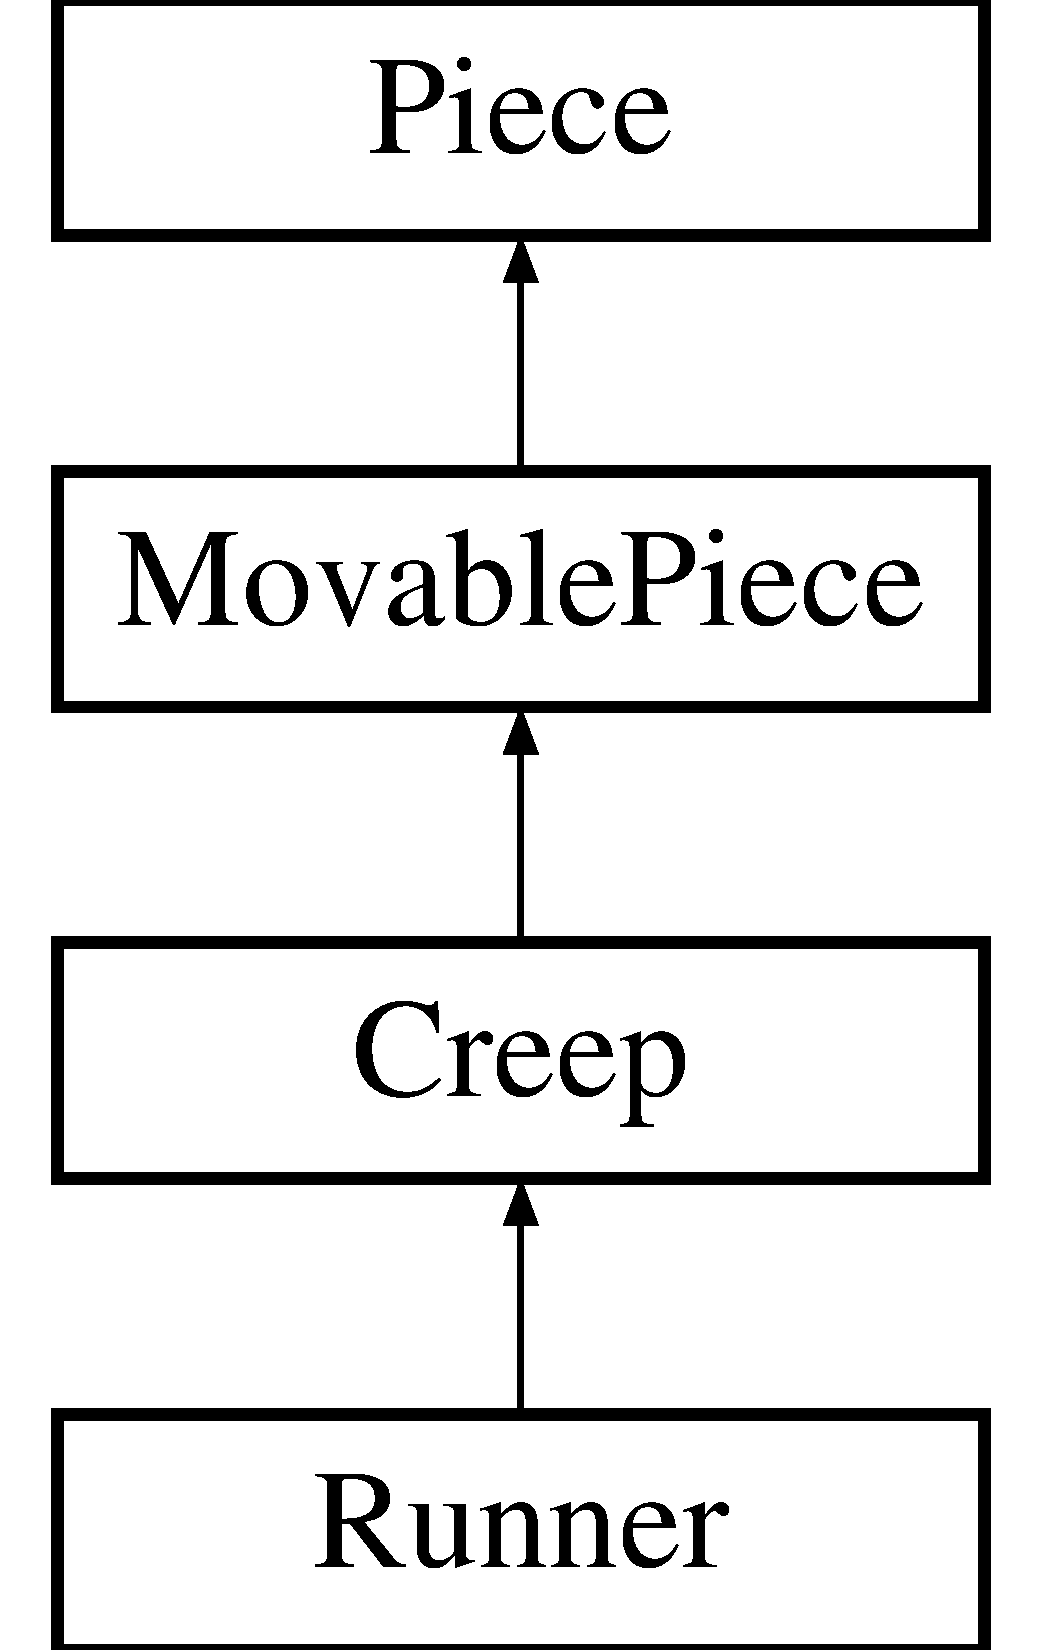
\includegraphics[height=4.000000cm]{classRunner}
\end{center}
\end{figure}


The documentation for this class was generated from the following file\-:\begin{DoxyCompactItemize}
\item 
/home/tom/\-Documents/\-Dev/\-C\-O\-S110\-\_\-\-Project/src/Runner.\-h\end{DoxyCompactItemize}

\hypertarget{classSleeper}{\section{Sleeper Class Reference}
\label{classSleeper}\index{Sleeper@{Sleeper}}
}
Inheritance diagram for Sleeper\-:\begin{figure}[H]
\begin{center}
\leavevmode
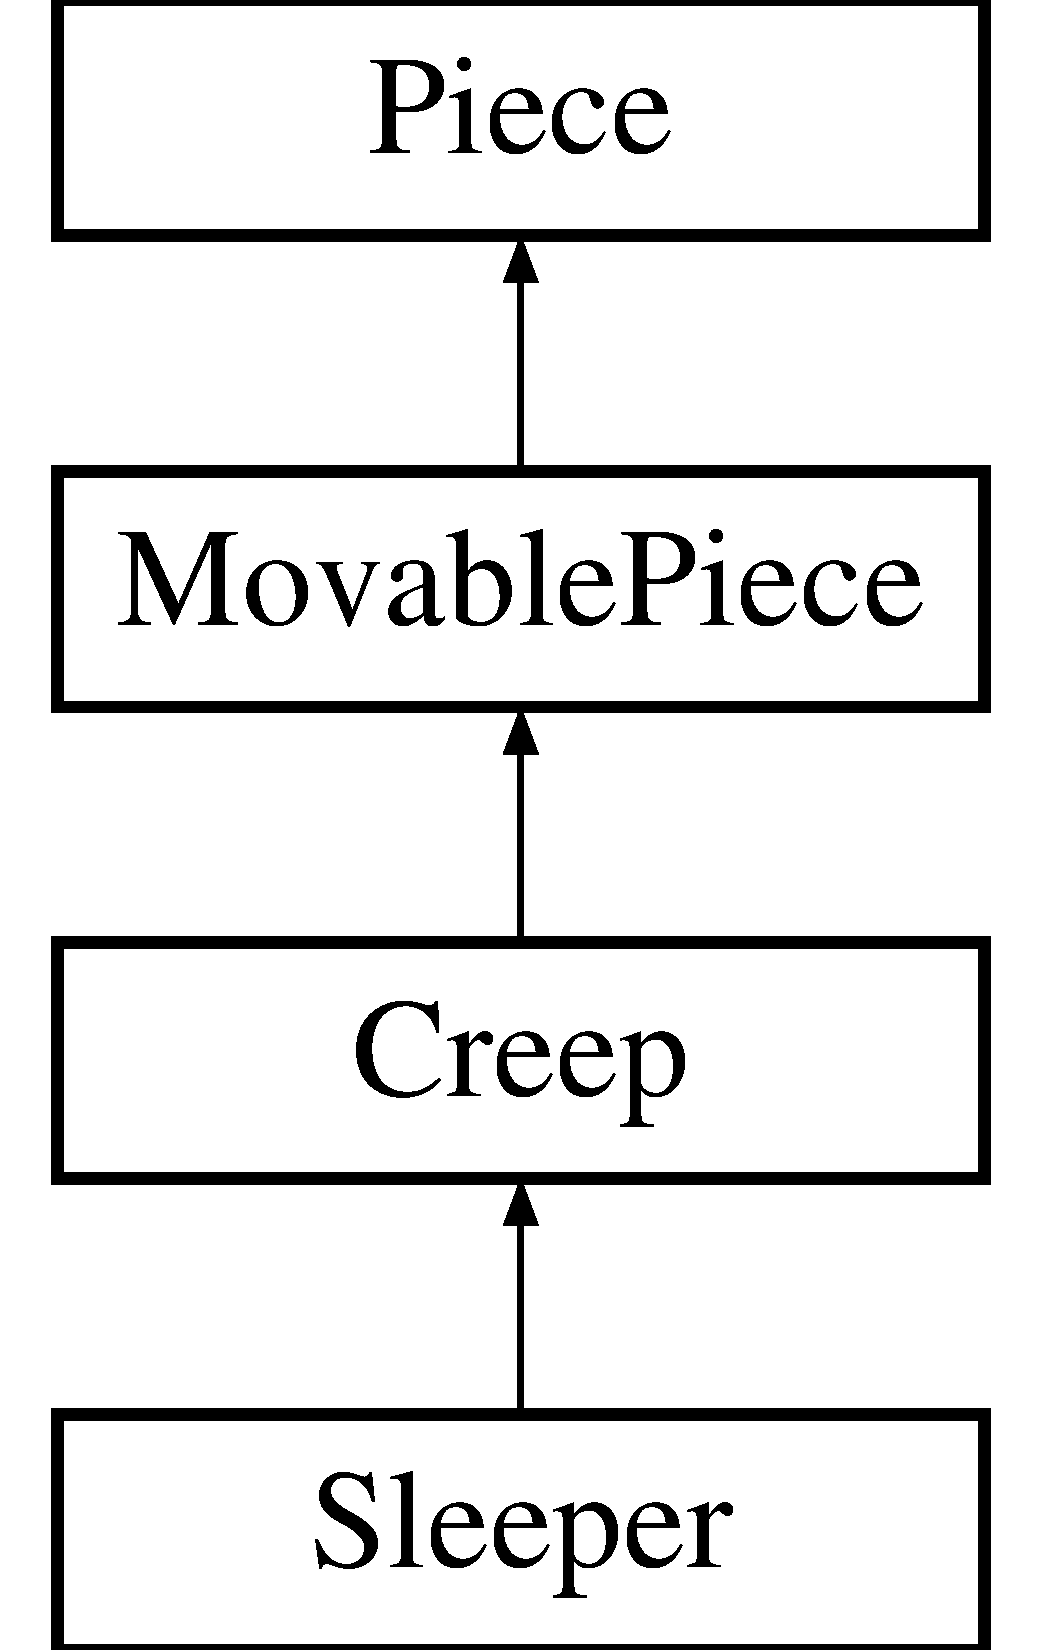
\includegraphics[height=4.000000cm]{classSleeper}
\end{center}
\end{figure}


The documentation for this class was generated from the following file\-:\begin{DoxyCompactItemize}
\item 
/home/tom/\-Documents/\-Dev/\-C\-O\-S110\-\_\-\-Project/src/Sleeper.\-h\end{DoxyCompactItemize}

\hypertarget{classSprite}{\section{Sprite Class Reference}
\label{classSprite}\index{Sprite@{Sprite}}
}
Inheritance diagram for Sprite\-:\begin{figure}[H]
\begin{center}
\leavevmode
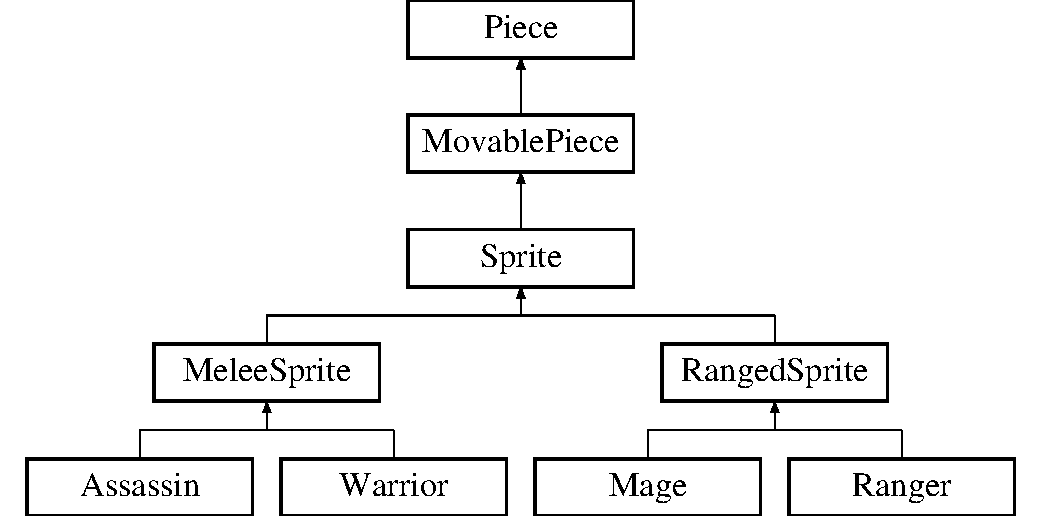
\includegraphics[height=5.000000cm]{classSprite}
\end{center}
\end{figure}


The documentation for this class was generated from the following file\-:\begin{DoxyCompactItemize}
\item 
/home/tom/\-Documents/\-Dev/\-C\-O\-S110\-\_\-\-Project/src/Sprite.\-h\end{DoxyCompactItemize}

\hypertarget{classWall}{\section{Wall Class Reference}
\label{classWall}\index{Wall@{Wall}}
}
Inheritance diagram for Wall\-:\begin{figure}[H]
\begin{center}
\leavevmode
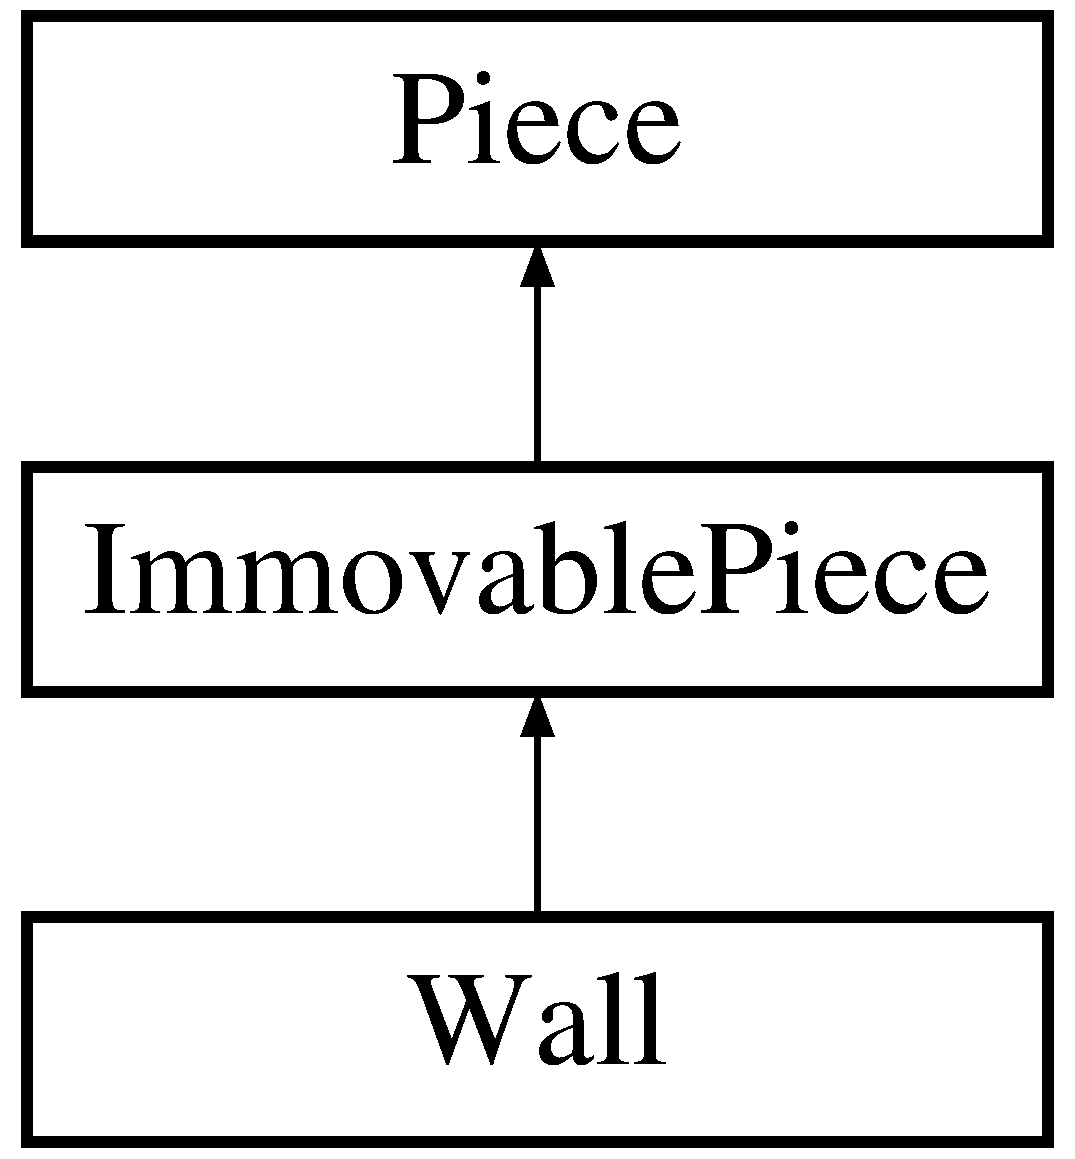
\includegraphics[height=3.000000cm]{classWall}
\end{center}
\end{figure}


The documentation for this class was generated from the following file\-:\begin{DoxyCompactItemize}
\item 
/home/tom/\-Documents/\-Dev/\-C\-O\-S110\-\_\-\-Project/src/Wall.\-h\end{DoxyCompactItemize}

\hypertarget{classWarrior}{\section{Warrior Class Reference}
\label{classWarrior}\index{Warrior@{Warrior}}
}
Inheritance diagram for Warrior\-:\begin{figure}[H]
\begin{center}
\leavevmode
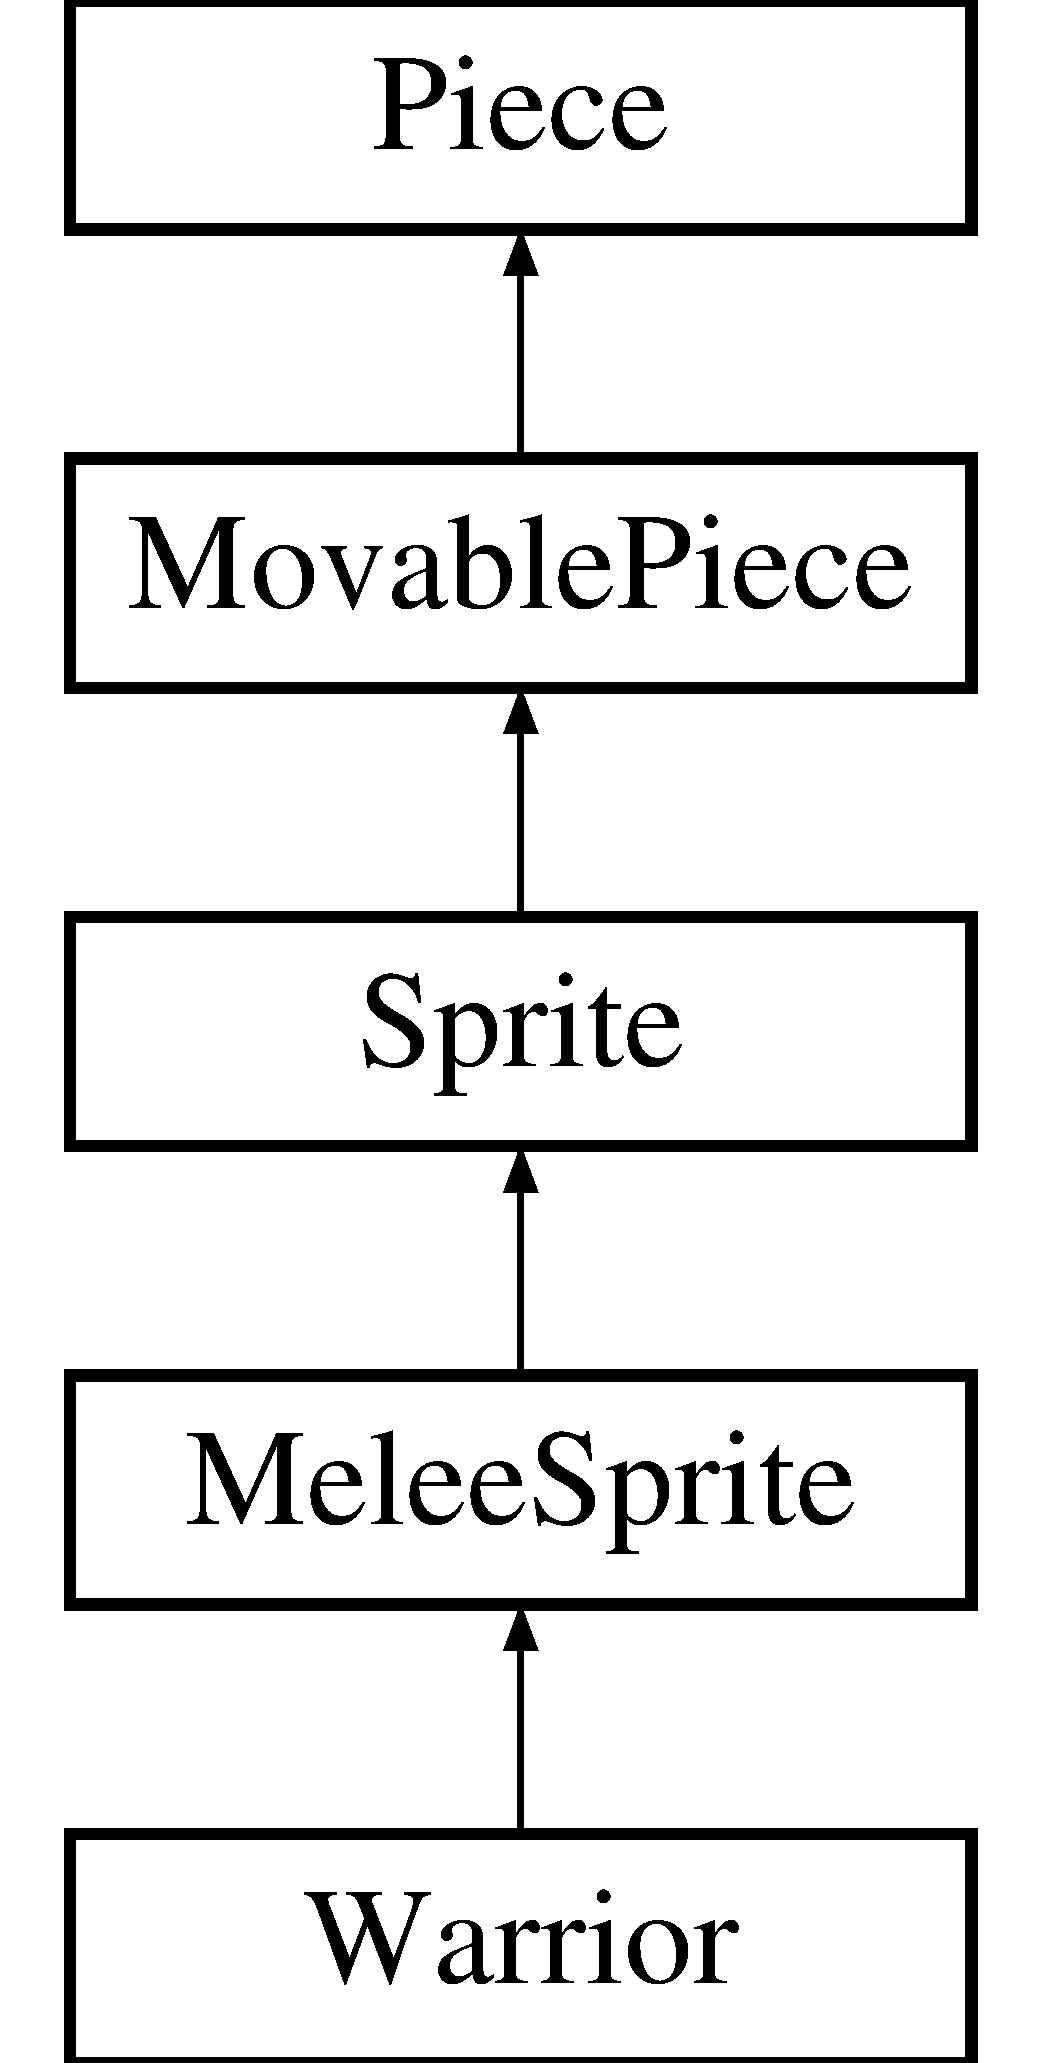
\includegraphics[height=5.000000cm]{classWarrior}
\end{center}
\end{figure}


The documentation for this class was generated from the following file\-:\begin{DoxyCompactItemize}
\item 
/home/tom/\-Documents/\-Dev/\-C\-O\-S110\-\_\-\-Project/src/Warrior.\-h\end{DoxyCompactItemize}

\hypertarget{classWaypoint}{\section{Waypoint Class Reference}
\label{classWaypoint}\index{Waypoint@{Waypoint}}
}
Inheritance diagram for Waypoint\-:\begin{figure}[H]
\begin{center}
\leavevmode
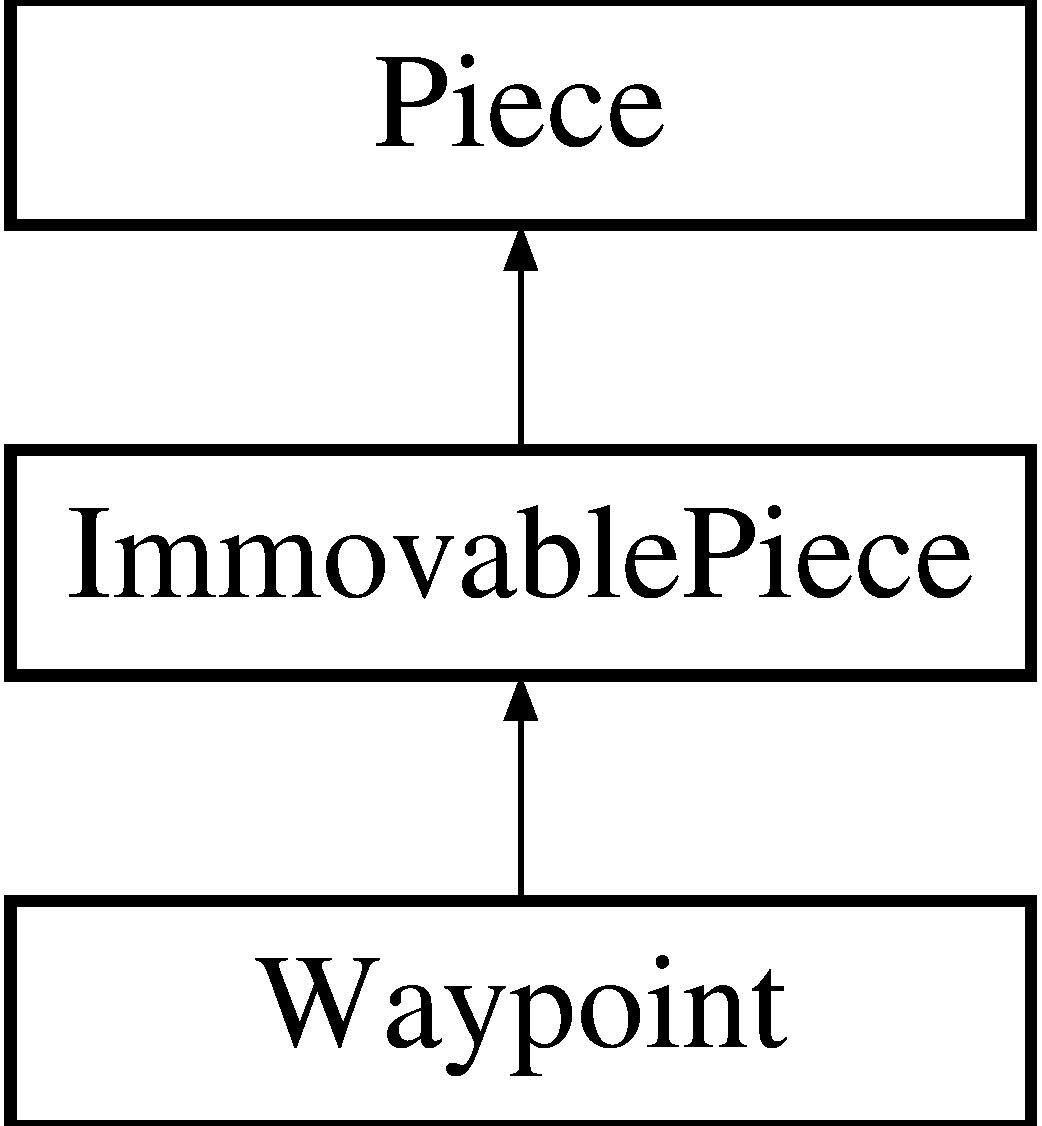
\includegraphics[height=3.000000cm]{classWaypoint}
\end{center}
\end{figure}


The documentation for this class was generated from the following file\-:\begin{DoxyCompactItemize}
\item 
/home/tom/\-Documents/\-Dev/\-C\-O\-S110\-\_\-\-Project/src/Waypoint.\-h\end{DoxyCompactItemize}

\addcontentsline{toc}{part}{Index}
\printindex
\end{document}
